Let the tens digit of the required number be ${a_1}$ and the units digit be ${a_0}$. Then
\begin{align}
    {a_1}+{a_0}=12
\end{align}
Which can be expressed as,
\begin{align}
     \myvec{1&1}\vec{x}=12\label{2006/1/b/eq1}
\end{align}
where
\begin{align}
    \vec{x}=\myvec{a_1\\a_0}
\end{align} 
Thus, the desired number  is 
\begin{align}
(10{a_1}+{a_0}) = 
    \myvec{10&1}\vec{x}
\end{align}
and the Number obtained by reversing the digits is
\begin{align}
    \myvec{1&10}\vec{x}
\end{align}
From the given information,  
\begin{align}
  \implies\myvec{10&1}\vec{x}-\myvec{1&10}\vec{x}&=18\\
   \implies\myvec{9&-9}\vec{x}&=18 \\ 
  \implies\myvec{1&-1}\vec{x}&=2\label{2006/1/b/eq2}
\end{align}
   \eqref{2006/1/b/eq1}and \eqref{2006/1/b/eq2} can be expressed as the matrix equation
 \begin{align}
    \myvec{
    1 & 1 \\-1 & 1}\vec{x} = \myvec{12\\2}
 \end{align}
 %
The augmented matrix for the above equation
is row reduced as follows
\begin{align}
\myvec{1&1&12\\-1&1&2}\xleftrightarrow{R_2\leftarrow R_2+ R_1} \myvec{1&1&12\\0&2&14}
\\
\xleftrightarrow{R_2\leftarrow \frac{1}{2}R_2} \myvec{1&1&12 \\ 0&1&7}
\\
\xleftrightarrow{R_1 \leftarrow R_1-R_2}
\myvec{1&0&5\\0&1&7}
\end{align}
yielding 
 \begin{align}
{a_1}&=5, {a_0}=7
\implies 
        10 {a_1}+{a_0}
        &=57
    \end{align}
    Fig. \ref{2006/1/b/Fig:Graphical Solution} verifies the solution .
  %
\begin{figure}[!ht]
    \centering
    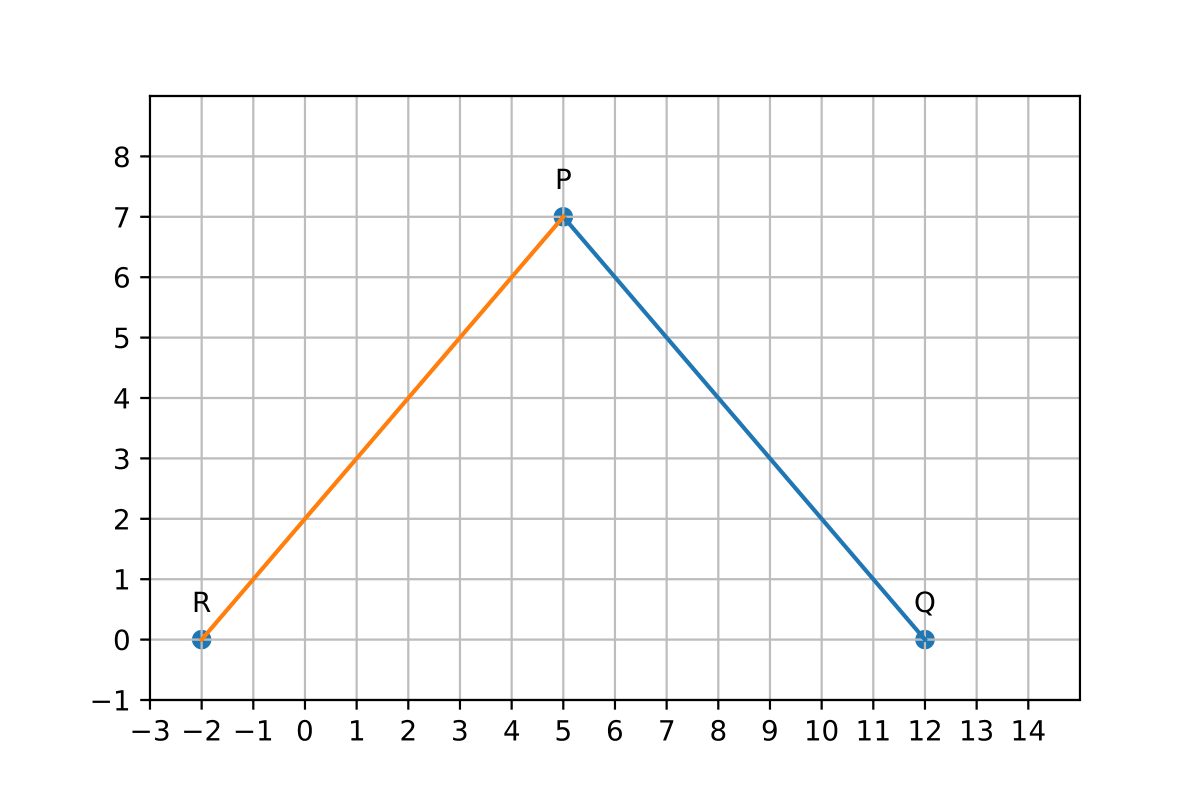
\includegraphics[width= \columnwidth]{linear_forms/solutions/1/b/Figure.png}
    \caption{Graphical solution}
    \label{2006/1/b/Fig:Graphical Solution}
\end{figure}
